\paragraph{Sơ đồ tuần tự luồng xác nhận email kích hoạt tài khoản}

Luồng nghiệp vụ này mô tả
quá trình người dùng nhấp
vào liên kết xác thực từ hòm thư điện tử cá nhân
để kích hoạt tài khoản,
chuyển hướng qua API Gateway.
nhận token JWT
và tiếp tục hoàn tất bước xác thực MFA trước khi truy cập hệ thống.

\begin{figure}[H]
\centering
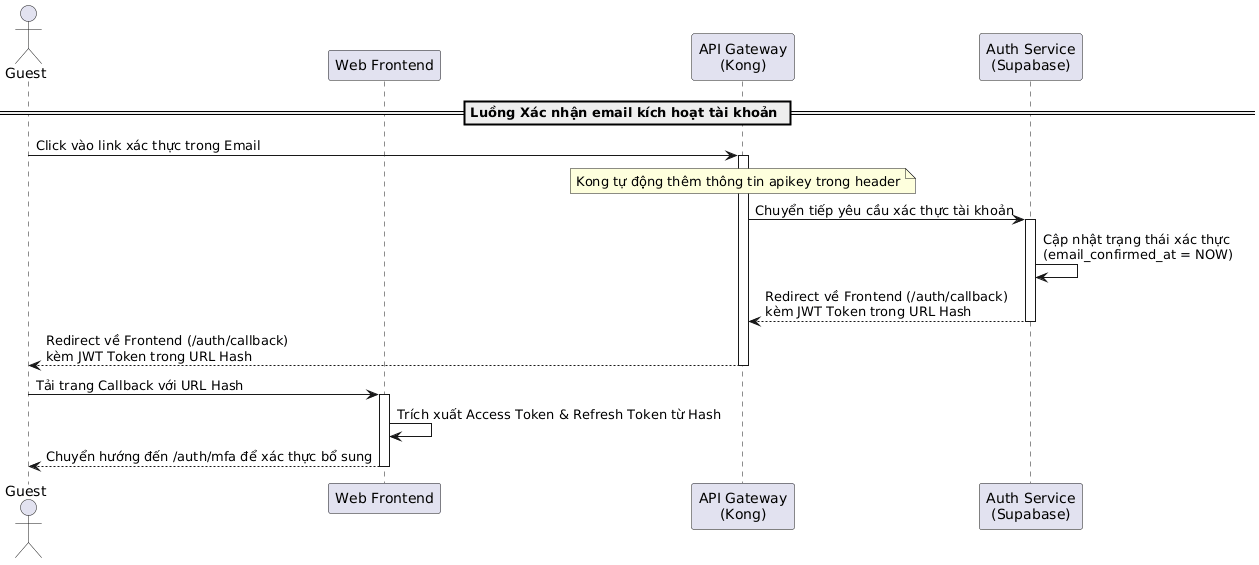
\includegraphics[width=0.95\textwidth]{contents/Sequence/UML-Sequence-GuestEmailConfirmation.png}
\caption{Sơ đồ tuần tự luồng xác nhận email kích hoạt tài khoản}
\end{figure}

\begin{table}[H]
\centering
\renewcommand{\arraystretch}{1.3}

\begin{tabular}{|l|l|p{5cm}|}
\hline
\textbf{Thành phần} & \textbf{Phân loại} & \textbf{Vai trò trong hệ thống} \\ \hline
Guest & Actor & Khách vãng lai thực hiện nhấp chọn liên kết xác thực. \\ \hline
Web Frontend & Component & Giao diện web Next.js. \\ \hline
API Gateway (Kong) & Component & Cổng API chuyển tiếp các yêu cầu API. \\ \hline
Auth Service (Supabase) & Microservice & Dịch vụ xác thực cập nhật trạng thái xác thực tài khoản và cấp JWT qua luồng redirect. \\ \hline
\end{tabular}
\caption{Các thành phần tham gia luồng xác nhận email kích hoạt tài khoản}
\end{table}

\subparagraph{Mô tả tổng quan}

\begin{itemize}

\item \textbf{Nhấp liên kết xác thực:}
Khách vãng lai mở thư cá nhân
và nhấn vào đường dẫn xác thực được gửi từ hệ thống.

\item \textbf{Chuyển tiếp yêu cầu:}
Cổng API chuyển tiếp yêu cầu xác thực tài khoản tới Auth Service.

\item \textbf{Kích hoạt tài khoản:}
Auth Service kiểm tra tính hợp lệ của mã xác nhận
và cập nhật trạng thái kích hoạt tài khoản
bằng cách ghi nhận thời gian xác nhận thư điện tử thành công.

\item \textbf{Chuyển hướng đăng nhập:}
Sau khi kích hoạt thành công,
Auth Service gửi yêu cầu chuyển hướng trình duyệt của người dùng
về trang xử lý của giao diện kèm theo mã đăng nhập
và mã làm mới trong địa chỉ trang web.

\item \textbf{Lưu trữ mã đăng nhập:}
Giao diện trích xuất các mã đăng nhập,
lưu trữ cục bộ và
chuyển người dùng đến trang xác thực hai lớp
để hoàn thành các bước bảo mật bổ sung trước khi vào màn hình trò chuyện chính.
\end{itemize}
